\section{Zielsetzung}

Die Funktionsweise eines Diodenlasers wird im folgenden Versuch untersucht. Mit dem Diodenlaser wird das Transmissionsspektrum einer Rubidium-Probe untersucht. 

\section{Theorie}

\subsection{Aufbau und Funktionsweise}
Laser ist ein Akronym für \textit{Light amplification by stimulated emission of radiation}.
Ein allgemeiner Laser ist darauf ausgelegt kohärentes, monochromatisches Licht hoher Intensität zu erzeugen. Dabei werden Elektronen in einem Medium durch eine Pumpenergie aus dem Grundzustand in ein höheres Niveau befördert. Damit der Laser anfängt zu lasen muss eine Besetzungsinversion erzeugt werden. Diese ist erreicht, wenn mehr Elektronen in einem höheren Niveau sind als in dem Grundzustand. Da bei einem Zwei-Niveausystem im Grenzfall beide Niveaus mit derselben Wahrscheinlichkeit besetzt sind, wird dort nie eine Besetzungsinversion entstehen, somit wird ein Niveausystem mit drei oder mehr Niveaus benötigt. Durch zwei Spiegel werden die emittierten Photonen reflektiert und erneut durch das Medium geschickt. Dabei erzeugen sie mit jedem Mal weitere Photonen aufgrund der Besetzungsinversion. Dieser Vorgang wird induzierte Emission genannt. Zwischen den Spiegeln entstehen stehende Wellen, deren Wellenlänge von dem Medium und der Resonatorlänge abhängig sind. 
Einer der beiden Spiegel transmittiert einen kleinen Teil des Lichts, wodurch der Laserstrahl aus dem Resonator gelangen kann, sobald dieser genug verstärkt und stabil ist. Dieser Vorgang ist in Abb. \ref{abb:laser} dargestellt.

\begin{figure}
    \centering
    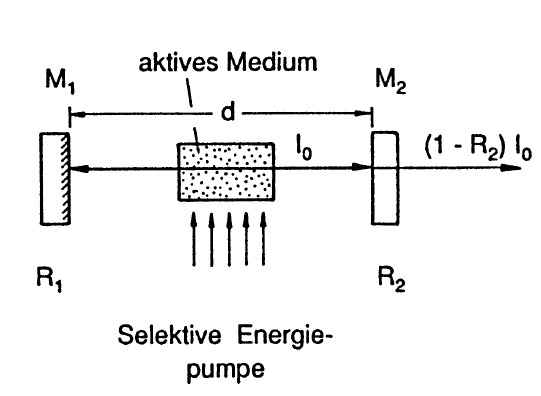
\includegraphics[width=0.5\textwidth]{pics/demtroeder.jpg}
    \caption{Der schematische Aufbau des Resonators eines Lasers. Das aktive Medium ist in der Mitte dargestellt. Daneben sind die Spiegel mit ihren jeweiligen Reflexionsfaktoren, wobei der rechte durchlässig ist und somit ein Anteil der Intensität transmittiert wird. \cite{demtroeder}}
    \label{abb:laser}
\end{figure}

Diodenlaser sind spezielle Laser, die aus einem Diodenchip und einem äußeren Gitter zusammengesetzt sind. 
Der Diodenchip besteht aus einer Halbleiter-Heterostruktur. Der Aufbau ist in Abb. \ref{abb:chip} dargestellt. Am oberen und unteren Ende sind jeweils Elektroden angebracht, die die Pumpenergie in Form von einem Anregungsstrom erbringen. Dadurch kommt es zur Rekombination eines Elektron-Loch-Paares in der aktiven Schicht. Die Energie, die durch die Rekombination, also in Abhängigkeit der Bandlücke entsteht, wird in Form von Photonen emittiert. Die Funktion des Resonators ist durch zwei planparallele Schichten gegeben. Alle anderen Grenzflächen sind rau um mögliche Oszillationen in anderen Schichten der Diode zu verhindern.  

\begin{figure}
    \centering
    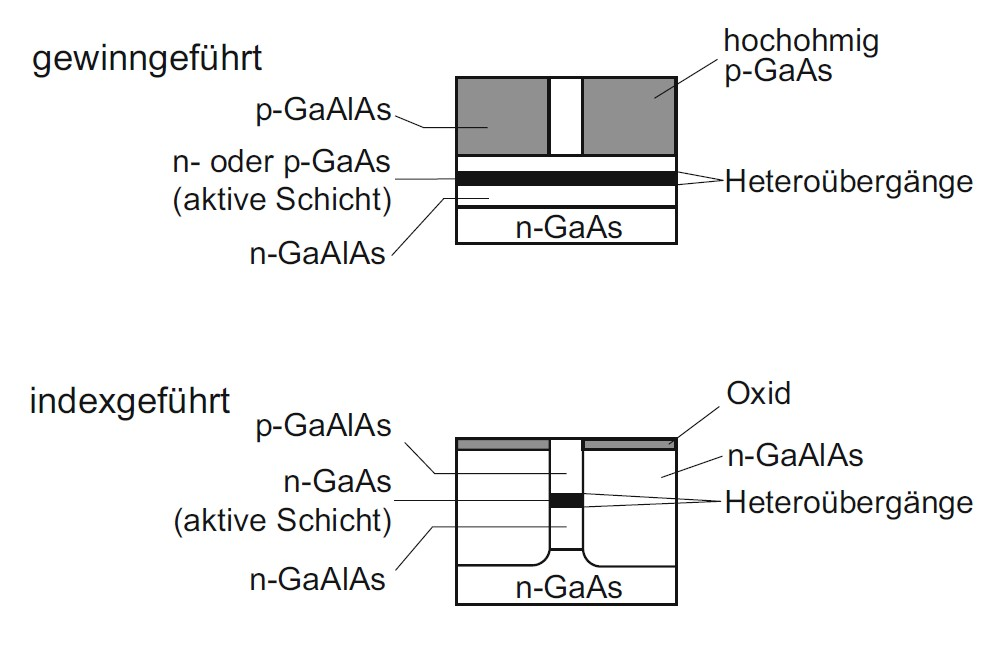
\includegraphics[width=0.6\textwidth]{pics/chip.jpg}
    \caption{Der Aufbau eines Diodenchips für typische Diodenlaser. Oben und unten an dem Chip sind Elektroden angeschlossen. \cite{eichler}}
    \label{abb:chip}
\end{figure}


Da die Form der Austrittsöffnung rechteckig ist, ist das emittierte Licht stark divergent. Durch eine Linse wird es kollimiert. Das Licht in diesem Experiment hat eine Wellenlänge in der Nähe von \SI{785}{\nm} bei einer Leistung von bis zu \SI{70}{\mW}. Die Linienbreite ist aber noch sehr groß, also im Bereich von \SI{50}{\MHz}, und damit ungeeignet für die Untersuchung atomarer Gegebenheiten. Außerdem ist die Frequenzstabilität empfindlich gegenüber Rückstreuung des Lichts in die Diode. Ein äußerer Resonator kann bei diesen Effekten helfen.
Der Resonator wird durch die zuvor beschriebene Linse und ein Beugungsgitter realisiert. Das Gitter kann sowohl vertikal als auch horizontal gedreht werden. Es besteht aus \num{1800} Linien$/$\si{\milli\metre}. Dabei werden \SI{85}{\percent} direkt reflektiert und nur \SI{15}{\percent} zurück in den Chip reflektiert, wodurch die Linienbreite auf weniger als \SI{1}{\MHz} zurückgeht. Das in die Diode reflektierte Licht trägt durch induzierte Emission zusätzlich zur Stabilität des Lasers bei. \cite{anleitung}

\subsection{Laserverstärkung}

Der Laser funktioniert meist auf der Frequenz mit der größten Verstärkung, da die stimulierte Emission das Lasen in anderen Moden begrenzt, sobald das Lasen einmal angefangen hat.
In Abb. \ref{abb:verstärker} ist die Verstärkung der verschiedenen Komponenten in Abhängigkeit der Wellenlänge aufgetragen. Die Verstärkung des aktiven Mediums ist materialabhängig, diese hängt nämlich von der Bandlücke des Halbleiters ab. Der daraus resultierende Peak ist sehr breit, da dieser primär von der Materialtemperatur abhängt.

\begin{figure}
    \centering
    \includegraphics[width=0.5\textwidth]{pics/verstärkung.jpg}
    \caption{Die einzelnen Verstärkungen des Diodenlasers in Abhängigkeit von der Wellenlänge. \cite{anleitung}}
    \label{abb:verstärker}
\end{figure}

Für eine Resonanz in der Rubidiumprobe muss die Temperatur so eingestellt werden, dass eine Wellenlänge von \SI{780}{\nm} erreicht wird. Auch der interne Resonator und seine Verstärkung hängen von der Temperatur ab. Außerdem ist er abhängig vom Anregungsstrom. Durch den Anregungsstrom ändert sich die Ladungsträgerdichte im aktiven Medium, wodurch sich der Brechungsindex $n$ ändert, was ebenfalls die Wellenlänge beeinflusst. In Abb. \ref{abb:temp} und \ref{abb:current} sind die Abhängigkeiten der Wellenlänge von der Temperatur und die Abhängigkeit vom Anregungsstrom für einen typischen Laser aufgetragen. Durch Einstellen des horizontalen Winkels des Beugungsgitters, lässt sich die Wellenlänge ebenfalls  nach der Bragg-Bedingung
\begin{equation*}
    \lambda = 2d \sin(\theta)
\end{equation*}
einstellen, wobei $d$ der Gitterkonstante entspricht und hier in etwa \SI{15}{\mm} beträgt. Insgesamt lässt sich die Wellenlänge also mithilfe der Temperatur, des Anregungsstroms und des Winkels und der Entfernung des Beugungsgitters einstellen.

\begin{figure}
    \begin{subfigure}{.5\textwidth}
      \centering
      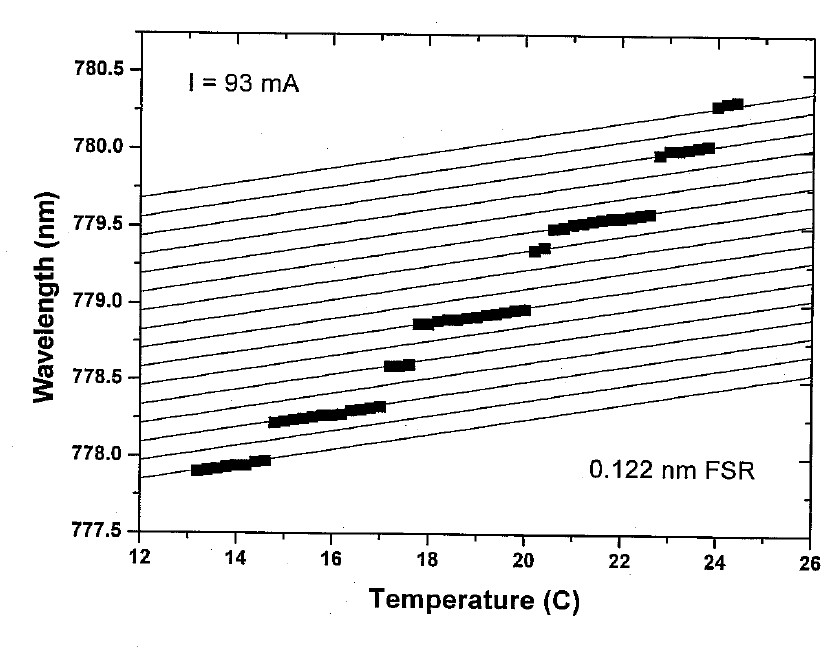
\includegraphics[width=0.8\linewidth]{pics/temperature.jpg}  
      \caption{Temperatur.}
      \label{abb:temp}
    \end{subfigure}
    \begin{subfigure}{.5\textwidth}
      \centering
      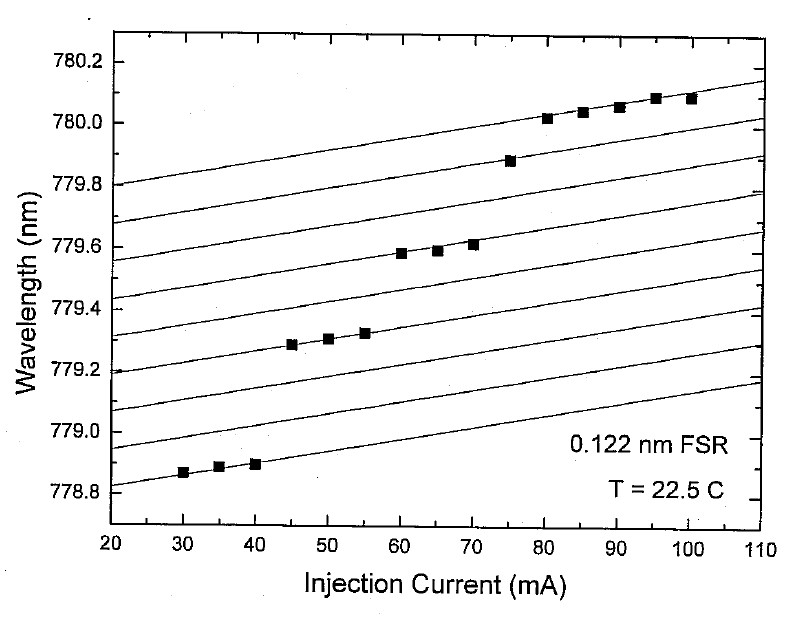
\includegraphics[width=0.8\linewidth]{pics/current.jpg}  
      \caption{Anregungsstrom.}
      \label{abb:current}
    \end{subfigure}
    \caption{Die Abhängigkeit der Wellenlänge ist hier jeweils einmal für die Temperatur des Diodenchips und einmal für den jeweils angelegte Anregungsstrom aufgetragen. \cite{anleitung}}
\label{fig:fig}
\end{figure}



\subsection{Rubidium Absorptionsspektrum}

Das vom Laser emittierte Licht mit einer erzwungenen Wellenlänge von \SI{780}{\nm} wird von der Rubidiumprobe absorbiert, da diese Wellenlänge der Übergangsenergie der Isotope entspricht. Die Übergänge sind in dem linken Teil der Abb. \ref{abb:Rb} dargestellt. Die Übergänge lassen sich dann durch die Variation der Spiegeleinstellungen sichtbar machen und sind als Senkungen der Transmission an verschiedenen Stellen zu erkennen. Dabei werden vier Peaks erwartet. Zwei vom $^{85}$Rb Isotop und zwei vom $^{87}$Rb Isotop. 

\begin{figure}
    \centering
    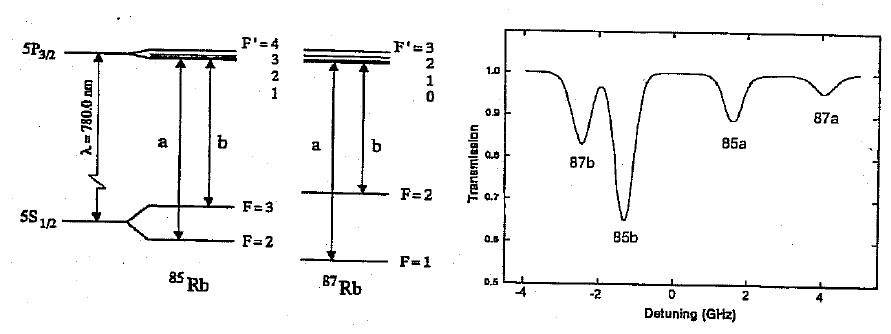
\includegraphics[width=0.9\textwidth]{pics/Rb_spectrum.jpg}
    \caption{Links sind die verantwortlichen Rb-Übergänge aufgetragen. Rechts ist das zu erwartende Spektrum der Transmission der Rb-Probe. \cite{anleitung}}
    \label{abb:Rb}
\end{figure}